\documentclass{article}
\usepackage{graphicx} % Required for inserting images
\usepackage[italian]{babel}
\usepackage{capt-of}
\usepackage[utf8]{inputenc}
\usepackage{flushend,stfloats,amsthm,chngpage,times,lipsum,lastpage} 

\begin{document}

\begin{titlepage}

\newcommand{\HRule}{\rule{\linewidth}{0.5mm}}

\center

\includegraphics[width=10cm]{unifi-logo.png}\\[1cm]

\center

\textsc{\LARGE Università degli Studi di Firenze}\\[0.5cm]
\textsc{\Large Dipartimento di Ingegneria dell'Informazione}\\[0.5cm] 

\makeatletter
\HRule \\[1cm]
{ \huge \bfseries Laboratorio di Algoritmi e Strutture Dati}\\[0.7cm]
\HRule \\[1.5cm]

\begin{minipage}{0.4\textwidth}
\begin{flushleft} \large
\emph{Autore:}\\
Francesca Sani % Your name
\\[1.2em]
\emph{N° Matricola:}\\
7025023 \\[1.2em]
\end{flushleft}
\end{minipage}
~
\begin{minipage}{0.4\textwidth}
\begin{flushright} \large
\emph{Corso principale:} \\
Algoritmi e Strutture Dati  \\[1.2em]
\emph{Docente corso:} \\
Simone Marinai
\end{flushright}
\end{minipage}\\[2cm]
\makeatother


\vfill

\end{titlepage}

\pagenumbering{gobble}

\newpage

\pagenumbering{arabic}

\tableofcontents

\newpage

\section{Introduzione}
Questa relazione ha l'obiettivo di confrontare vari modi per calcolare la \textbf{Longest Common Subsequence} (\textit{LCS}) tra due stringhe, in modo da comprendere i vantaggi e gli svantaggi delle diverse implementazioni.
$\\$
$\\$
Verranno analizzati gli algoritmi di \textbf{ "forza-bruta"}, la versione \textbf{ricorsiva}, la versione ricorsiva con \textbf{memoization} e infine la versione \textbf{bottom-up}.

\subsection{Ambiente di test}
Il codice per eseguire gli esperimenti è stato realizzato in Python (interprete versione 3.9). L'ambiente di sviluppo è l'IDE PyCharm 2023.1.2.
$\\$
$\\$
Il computer su cui è stato scritto il codice ha le seguenti specifiche: MacBook Air Chip Apple M2 con CPU 8-core, 16GB di memoria unificata e sistema operativo macOS Ventura 13.6.
$\\$
$\\$
La relazione è stata scritta in \LaTeX \  tramite l'utilizzo dell'editor online \textit{Overleaf}.

\subsection{Librerie utilizzate}
Il programma Python scritto utilizza le seguenti librerie:
\begin{itemize}
    \item \textbf{numpy}: permette di lavorare su tempi calcolati e metterli nella tabella generata;
    \item \textbf{timeit}: permette di misurare i tempi di esecuzione dei vari algoritmi;
    \item \textbf{matplotlib}: permette di generare grafici e tabelle, in modo da poter analizzare al meglio le prestazioni degli algoritmi;
    \item \textbf{random} e \textbf{string}: permettono di generare sequenze di stringhe casuali;
    \item \textbf{intertools} e \textbf{combinations}, permettono di ottenere tutte le sottosequenze della sequenza passata.
\end{itemize}

\newpage

\section{Cenni teorici}

\subsection{Problema della Longest Common Subsequence}
Una sottosequenza di una data sequenza è la sequenza stessa alla quale tolgo zero o più elementi. Formalmente, data una sequenza $X = <x_1, x_2, ... , x_m>$, un'altra sequenza $Z = <z_1, z_2, ... , z_k>$ è una \textbf{sottosequenza} di X se $\exists$ una sequenza di indici $I = <i_1, i_2, ... , i_k>$ tale che $\forall j = 1, 2, ..., k$ si ha $x_{ij} = z_j$.
$\\$
$\\$
Date due sequenze X e Y, diciamo che una sequenza Z è una \textbf{sottosequenza comune} di X e Y se Z è una sottosequenza di X e Y. 
$\\$
$\\$
Nel problema della \textbf{LCS}, date due sequenze $X = <x_1, x_2, ... , x_m>$ e $\\$ $Y = <y_1, y_2, ... , y_n>$, si desidera trovare una sottosequenza comune di lunghezza massima comune a X e Y.

\begin{center}
    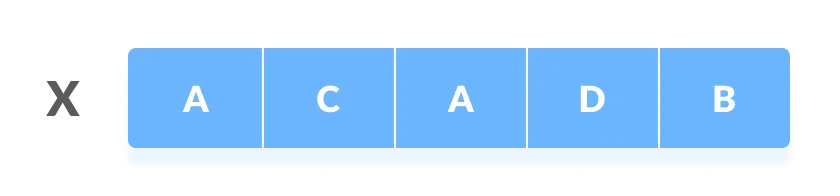
\includegraphics[width=160px]{LCS/s1.png}
    \captionof{figure}{Sequenza X data in ingresso}
    \medskip
    \medskip
    
\includegraphics[width=150px]{LCS/s2.png}
    \captionof{figure}{Sequenza Y data in ingresso}
    \medskip
    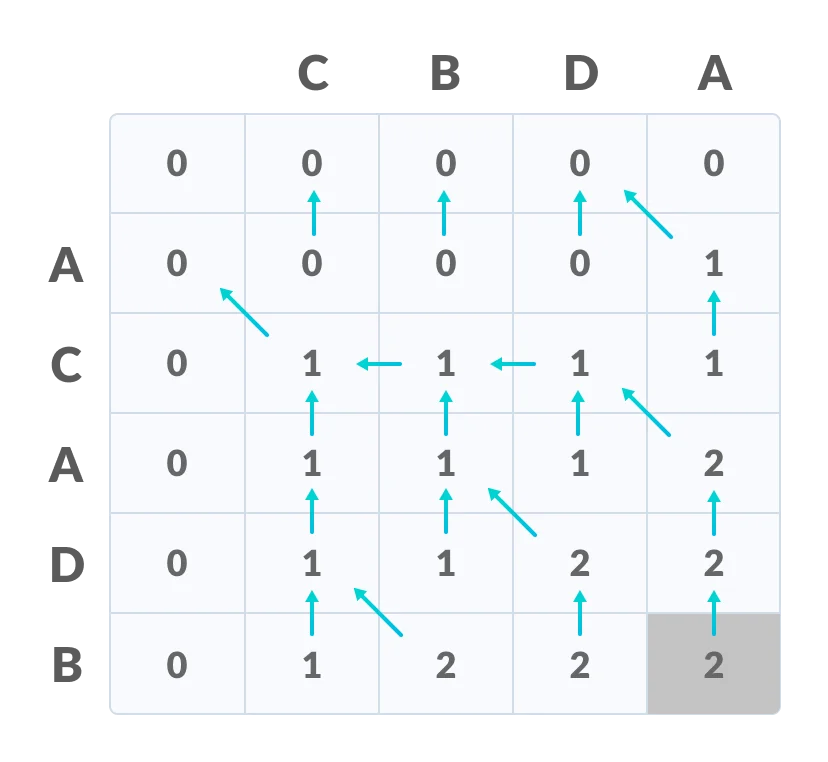
\includegraphics[width=130px]{LCS/tab-lcs.png}
    \captionof{figure}{Tabella generata per calcolare la LCS}
    \medskip
    
\includegraphics[width=80px]{LCS/lcs.png}
    \captionof{figure}{Sottosequenza comune delle sequenze X e Y}
\end{center}

\subsection{Algoritmo "forza-bruta"}

In un approccio di \textbf{forza-bruta} per risolvere il problema LCS, enumeriamo tutte le sottosequenze di X e controlliamo ogni sottosequenza per vedere se è anche una sottosequenza di Y, tenendo traccia della sottosequenza più lunga che troviamo.
$\\$
Dato che X ha $2^m$ sottosequenze, questo approccio richiede un \textit{tempo esponenziale}, rendendolo impraticabile per sequenze lunghe.

\subsubsection{Teorema - Sottostruttura ottimale di un LCS}

Date le sequenze $X = <x_1, x_2, ... , x_m>$ e $Y = <y_1, y_2, ... , y_n>$. $\\$ Sia $Z = <z_1, z_2, ... , z_k>$ una qualsiasi LCS di X e Y.
\begin{itemize}
    \item Se $x_m = y_n$, allora $z_k = x_m = y_n$ e $Z_{k-1}$ è una LCS di $X_{m-1}$ e $Y_{n-1}$.
    \item Se $x_m \neq y_n$, allora $z_k \neq x_m$ implica che $Z$ è una LCS di $X_{m-1}$ e $Y$.
    \item Se $x_m \neq y_n$, allora $z_k \neq y_n$ implica che $Z$ è una LCS di $X$ e $Y_{n-1}$.
\end{itemize}

\subsection{Versione ricorsiva}

Il teorema implica che ci siano uno o due sottoproblemi da esaminare per trovare una LCS di X e Y. 
$\\$
Se $x_m = y_n$, abbiamo trovato \textit{una} LCS di $X_{m-1}$ e $Y_{n-1}$.
$\\$
Se $x_m \neq y_n$, allora dobbiamo risolvere \textit{due} sottoproblemi: trovare una LCS di $X_{m-1}$ e $Y$, e trovare una LCS di $X$ e $Y_{n-1}$. La più lunga di queste due LCS è una LCS di X e Y.
$\\$
$\\$
La soluzione \textbf{ricorsiva} richiede la definizione di una ricorrenza per il valore di una soluzione ottima.
$\\$
Definiamo $c[i, j]$ come la lunghezza di una LCS delle sequenze $X_i$ e $Y_j$. Se $i = 0$ o $j = 0$, una delle sequenze ha lunghezza 0. La sottostruttura ottima del problema della LCS consente di scrivere la seguente formula ricorsiva:
$\\$
$\\$
$c[i, j] =\left\{
\begin{array}{rcrcrcr}
0\ \ \ \ \ \ \ \ \ \ \ \ \ \ \ \ \ \ \ \ \ \ \ \ \ \ \ \ \ \ \ \ \ \ \ \ \ \ \ \ \ \ \ \ &&&se\ i = 0\ o\ j = 0\\
c[i-1, j-1]+1\ \ \ \ \ \ \ \ \ \ \ \ \ \ \ \ &&&\ se\ i, j > 0\ x_i = y_j\\
max(c[i, j-1], c[i-1, j])&&&\ se\ i, j > 0\ x_i \neq y_j\\
\end{array}
\right.$
$\\$
$\\$
$\\$
Anche questa implementazione, nonostante sia semplice, è inefficiente a causa della sovrapposizione nei sottoproblemi, pertanto la complessità temporale resta esponenziale. 

\subsection{Versione ricorsiva con memoization}

Per evitare la sovrapposizione dei sottoproblemi, attraverso la \textbf{memoization}, è possibile memorizzare i risultati ottenuti in una tabella, in modo da non doverli calcolare più volte.
$\\$
$\\$
Questo permette di migliorare notevolmente le prestazioni dell'algoritmo (rispetto alla versione di forza-bruta e alla versione ricorsiva), ma a causa della presenza della ricorsione può non essere molto efficiente quando si hanno input di grandi dimensioni.

\subsection{Versione bottom-up}

Un'altra soluzione, dato che ci sono $\Theta(mn)$ sottoproblemi distinti, è quella di utilizzare la \textit{programmazione dinamica} per calcolare le soluzioni con un metodo \textbf{bottom-up}.
$\\$
$\\$
Date due sequenze in input, memorizza i valori $c[i][j]$ in una tabella $c[0...m][0...n]$, le cui posizioni sono calcolate secondo l'ordine delle righe. Il tempo di esecuzione è $O(mn)$, perché il calcolo di ogni posizione della tabella richiede un tempo $\Theta(1)$.

\subsection{Prestazioni attese}

Questa relazione, come detto in precedenza, ha l'obiettivo di confrontare le prestazioni di quattro diverse implementazioni di "calcolo" per trovare la più lunga sottosequenza comune tra due stringhe.
$\\$
Quello che ci si aspetta dai test eseguiti, e commentati nelle sezioni successive, è che il metodo migliore per ricavare la LCS sia l'approccio \textit{bottom-up}.
$\\$
$\\$
Le varie complessità temporali si possono distinguere come segue:
\begin{itemize}
    \item \textbf{Approccio di forza-bruta}, poiché si esaminano tutte le sottosequenze di X e si verifica se sono sottosequenze di Y, ci aspettiamo una complessità esponenziale $O(2^m * n)$;
    \item \textbf{Approccio ricorsivo}, poiché vengono considerate tutte le possibili sottosequenze di X e Y, ci aspettiamo una complessità esponenziale $O(2^{m+n})$;
    \item \textbf{Approccio ricorsivo con memoization}, grazie alla memorizzazione dei sottoproblemi già analizzati permette di ridurre notevolmente la complessità, che non sarà più esponenziale $O(mn)$;
    \item \textbf{Approccio bottom-up}, le lunghezze delle sottosequenze analizzate vengono memorizzate in una tabella, avendo così una complessità $O(mn)$.
\end{itemize}

$\\$

\begin{center}
    \begin{tabular}{|l|c|c|r|}
        \hline
        \multicolumn{2}{|c|}{\textbf{Algoritmo}} & \multicolumn{2}{c|}{\textbf{Complessità}}\\
        \hline
        \multicolumn{2}{|c|}{Forza-Bruta} & \multicolumn{2}{c|}{$O(2^m * n)$}\\
        \multicolumn{2}{|c|}{Ricorsivo} & \multicolumn{2}{c|}{$O(2^{m + n})$}\\
        \multicolumn{2}{|c|}{Ricorsivo con Memoization} & \multicolumn{2}{c|}{$O(mn)$}\\
        \multicolumn{2}{|c|}{Bottom-Up} & \multicolumn{2}{c|}{$O(mn)$}\\
        \hline
    \end{tabular}
    \captionof{table}{Complessità temporale per LCS}
\end{center}

\newpage

\section{Documentazione del codice}

Per svolgere i vari test è stato scritto codice in Python, ovvero sono stati definiti vari metodi che permettono di calcolare la LCS con i diversi algoritmi in esame, generare grafici e tabelle, etc.

\subsection{Descrizione dei metodi implementati}

In questa sezione vengono spiegate le funzionalità di ogni metodo che è possibile trovare nel file \textbf{main.py}.


\begin{itemize}
    \item $lcs\_bruteForce(s1,\ s2)$ : metodo per l'algoritmo di forza-bruta, in cui vengono create tutte le sottosequenze della stringa s1 e per ciascuna si effettua un confronto per carattere con l'altra stringa s2, questo metodo ritorna la lunghezza della LCS trovata;
    \item $allSubsequences(s)$ : metodo che viene chiamato da $lcs\_bruteForce(s1,\ s2)$ per generare tutte le sottosequenze possibili della stringa s;
    \item $lcs\_recursive(s1,\ s2)$ e $recursive(s1,\ s2,\ m,\ n)$ : metodi per l'algoritmo ricorsivo, $lcs\_recursive(s1,\ s2)$ date due stringhe permette di entrare nella vera e propria ricorsione, invece $recursive(s1,\ s2,\ m,\ n)$ date le due stringhe e le loro dimensioni calcola la LCS secondo la formula ricorsiva definita precedentemente; 
    \item $lcs\_memoization(s1,\ s2)$ e $memoization(s1,\ s2,\ c,\ m,\ n)$ : metodi per l'algoritmo ricorsivo con memoization, $lcs\_memoization(s1,\ s2)$ date due stringhe permette di entrare nella vera e propria ricorsione e permette di generare la matrice di memorizzazione, invece $memoization(s1,\ s2,\ c,\ m,\ n)$ date le due stringhe, la matrice di memorizzazioni e le loro dimensioni calcola la LCS secondo la formula ricorsiva e verificando se un certo risultato è già stato calcolato;
    \item $lcs\_bottomUp(s1,\ s2)$: metodo per l'algoritmo bottom-up, in cui viene calcolata la LCS partendo dai primi caratteri delle stringhe e memorizzando i risultati in una matrice; 
    \item $stringGenerator(length)$: metodo per generare delle sequenze di stringhe casuali;
    \item $measureTime(function, s1, s2)$: metodo per calcolare i tempi medi della funzione data;
    \item $drawPlots()$: metodo per generare grafici;
    \item $drawTable(columns, headers, title)$: metodo per generare tabelle;
    \item $test()$: metodo chiamato dal $main()$ per eseguire i test, il quale a sua volta chiama quasi tutti i metodi definiti in precedenza.
\end{itemize}

\newpage

\section{Descrizione dei test}

Per eseguire i test sono state generate sequenze di stringhe casuali da 1 a 13 (attraverso la funzione \textit{stringGenerator(length)}), pertanto sono stati eseguiti 12 test e per rendere più attendibili i risultati ottenuti, ciascun test è stato eseguito 100 volte e poi è stata calcolata una media dei tempi di esecuzione.
$\\$
$\\$
I tempi di esecuzione sono stati calcolati attraverso l'uso del metodo fornito dal modulo di Python \textit{timeit}: \textbf{\textit{timeit(stmt, number)}}. Questo metodo, chiamato nella funzione \textit{measureTime(function, s1, s2)} restituisce il tempo totale ottenuto per l'esecuzione dei test.

\subsection{Grafici dei tempi di esecuzione}

Di seguito sono riportati i grafici che, al variare della lunghezza delle stringhe confrontate, mostrano l'andamento dei tempi di esecuzione per ciascun algoritmo in esame.
$\\$
Inoltre, è riportato un grafico che racchiude i 4 grafici singoli, in modo da poter avere un confronto più accurato.

\begin{center}
    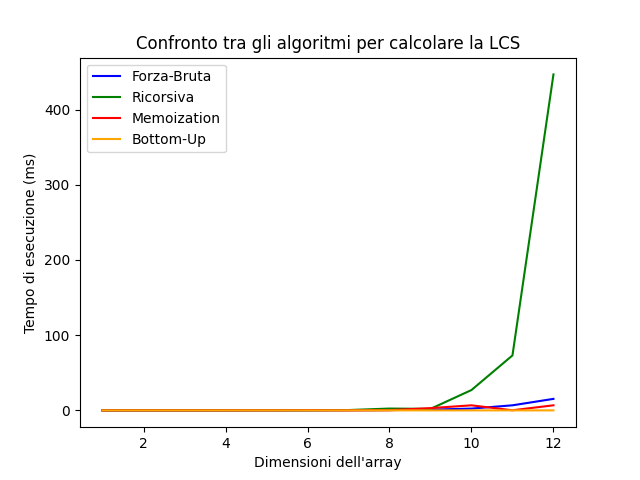
\includegraphics[width=290px]{plots/GraficoLCS.png}
    \captionof{figure}{Tempi di esecuzione per calcolare la LCS}
\end{center}

\subsubsection{Algoritmo forza-bruta}
\begin{center}
    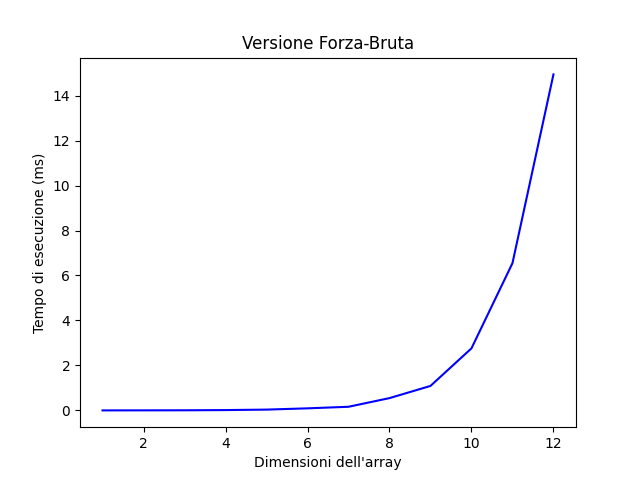
\includegraphics[width=290px]{plots/Forza-Bruta.png}
    \captionof{figure}{Tempi di esecuzione dell'algoritmo Forza-Bruta}
\end{center}

\subsubsection{Algoritmo ricorsivo}
\begin{center}
    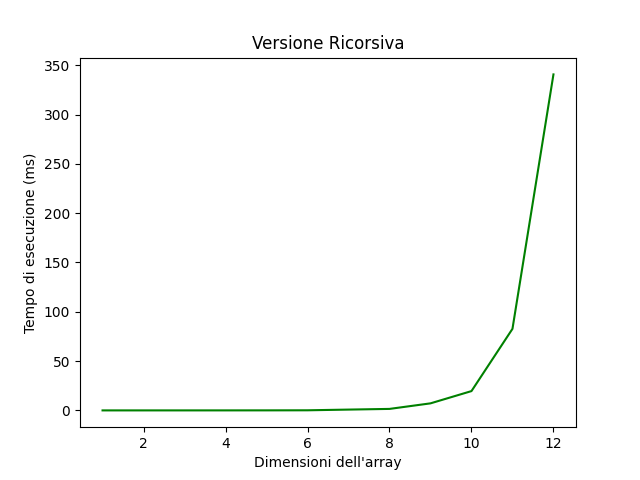
\includegraphics[width=290px]{plots/Ricorsiva.png}
    \captionof{figure}{Tempi di esecuzione dell'algoritmo Ricorsivo}
\end{center}

\subsubsection{Algoritmo ricorsivo con memoization}
\begin{center}
    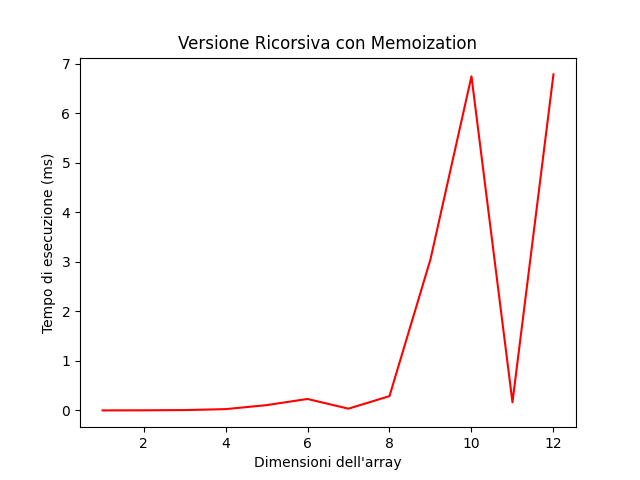
\includegraphics[width=290px]{plots/Memoization.png}
    \captionof{figure}{Tempi di esecuzione dell'algoritmo ricorsivo con Memoization}
\end{center}

\subsubsection{Algoritmo bottom-up}
\begin{center}
    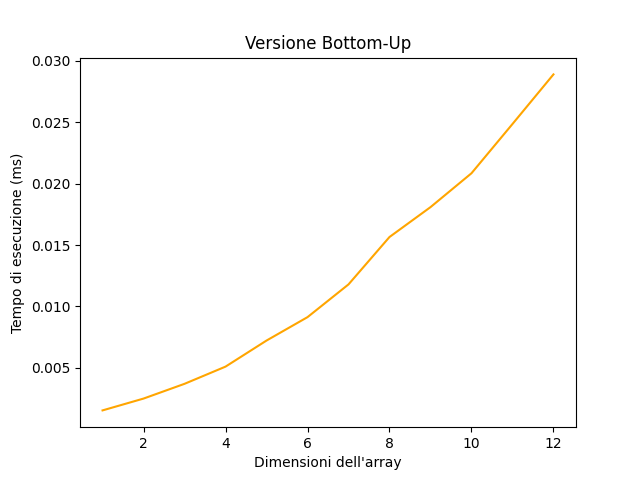
\includegraphics[width=300px]{plots/Bottom-Up.png}
    \captionof{figure}{Tempi di esecuzione dell'algoritmo Bottom-Up}
\end{center}


\subsection{Tabelle dei tempi di esecuzione}

Di seguito è riportata la tabella contenente i tempi di esecuzione dei quattro algoritmi analizzati, grazie ai quali è stato possibile generare i grafici della sezione precedente.

\begin{figure} [!h]
    \centering
    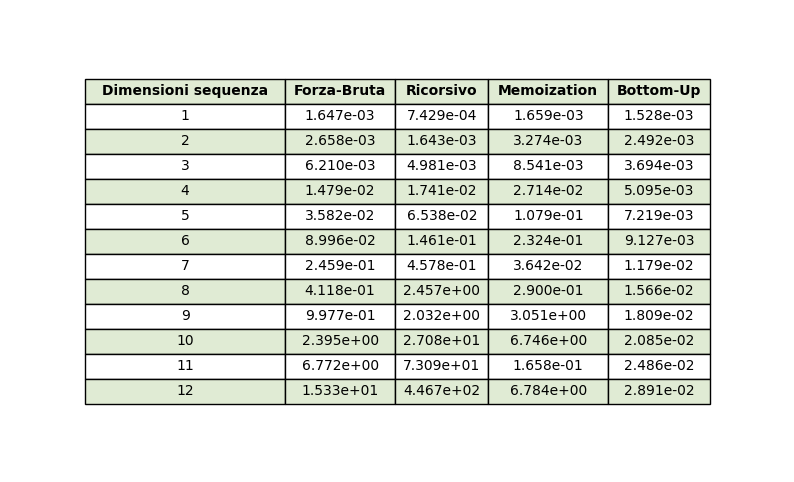
\includegraphics[width=1\linewidth]{table/TabellaLCS.png}
    \caption{Tabella dei tempi di esecuzione per calcolare la LCS}
    \label{fig:enter-label}
\end{figure}

\newpage

\section{Considerazioni finali}

In conclusione, osservando i risultati ottenuti dai vari test ed analizzando i grafici e la tabella, è stato possibile raggiungere l'obiettivo di questa relazione: confrontare quattro diverse implementazioni per calcolare la più lunga sottosequenza comune (LCS) tra due stringhe.
$\\$
$\\$
Dal grafico in \textit{figura 5} è possibile trarre una prima conclusione, ovvero che il metodo migliore per calcolare la LCS è quello bottom-up, invece l'approccio ricorsivo è quello peggiore.
$\\$
$\\$
Il grafico in \textit{figura 6} e quello in \textit{figura 7}, che rappresentano rispettivamente l'andamento dei tempi di esecuzione per l'algoritmo di forza-bruta e per quello ricorsivo, confermano che la loro complessità temporale è esponenziale.
$\\$
È interessante notare che, nonostante siano entrambi esponenziali, uno è migliore dell'altro. Infatti, anche se il metodo di forza-bruta a primo impatto possa sembrare peggiore, poiché esamina tutte le sottosequenze di X e controlla se esse sono presenti in Y, non è stato così.
$\\$
$\\$
Analogamente, il grafico in \textit{figura 8} e il grafico in \textit{figura 9}, i quali rappresentano rispettivamente l'andamento dei tempi di esecuzione per l'algoritmo ricorsivo con memoization e per quello bottom-up, confermano che la loro complessità temporale è quadratica.
$\\$
$\\$
Andando adesso ad analizzare la tabella in \textit{figura 10} è possibile confrontare direttamente i tempi di esecuzione dei quattro approcci in esame. Nonostante le dimensioni delle sequenze generate aumentino, i tempi di esecuzione di bottom-up sono quasi sempre minori. Infatti per piccole dimensioni delle sequenze (1/2 caratteri), gli approcci migliori sono quelli ricorsivo e di forza-bruta.
$\\$
È inoltre importante osservare che l'algoritmo ricorsivo con memoization, rispetto a quello ricorsivo e quello di forza-bruta, mostra notevoli vantaggi, nonostante il picco temporale che si verifica con dimensioni maggiori delle sequenze (circa 8/9 caratteri), osservabile anche nei grafici in \textit{figura 5} e \textit{8}.
$\\$
$\\$
In sintesi, è stato possibile affermare che grazie all'analisi condotta, ciò che era stato descritto nella sezione teorica, è confermato.

\newpage

\section{Bibliografia}

\textbf{Figura 1}: Programmiz - LCS
$\\$
$\\$
\textbf{Figura 2}: Programmiz - LCS
$\\$
$\\$
\textbf{Figura 3}: Programmiz - LCS
$\\$
$\\$
\textbf{Figura 4}: Programmiz - LCS


\end{document}
